% /**
%  * @file dokumentace.tex
%  * @author Dias Assatulla (xassat00@stud.fit.vutbr.cz)
%  * @author David Kvaček (xkvace00@stud.fit.vutbr.cz)
%  * @author Jakub Sychra (xsychr06@stud.fit.vutbr.cz)
%  * @author Tomáš Šedo (xsedot00@stud.fit.vutbr.cz)
%  * @brief Project documentation from IFJ and IAL courses.
%  * @date 2023-12-06
%  */

\documentclass[a4paper, 11pt]{article}
\usepackage[left=2cm, text={17cm, 25cm}, top=3cm]{geometry}
\usepackage[czech]{babel}
\usepackage[utf8]{inputenc}
\usepackage[IL2]{fontenc}
\usepackage{graphicx}
\usepackage{hyperref}
\usepackage{colortbl}

\begin{document}

\begin{titlepage}
    \begin{center}
        
\includegraphics[scale=0.125]{logo.png} \\
        \vspace{\stretch{0.382}}
        \LARGE{Dokumentace projektu z~předmětů IFJ a~IAL} \\
        \huge{\textbf{Implementace překladače imperativního jazyka~IFJ23}} \\
        \LARGE{Tým xsedot00, varianta vv-BVS} \\
        \LARGE{Rozšíření: \textbf{FUNEXP}}
        \vspace{\stretch{0.618}}
    \end{center}

    \null \hfill \Large{Dias Assatulla (xassat00)\,--\,25\,\%} \\
    \null \hfill \Large{David Kvaček (xkvace00)\,--\,25\,\%} \\
    \null \hfill \Large{Jakub Sychra (xsychr06)\,--\,25\,\%} \\
    \Large{Brno, \today \hfill \textbf{Tomáš Šedo (xsedot00)\,--\,25\,\%}}
\end{titlepage}

\tableofcontents

\newpage

\section{Úvod}
    V~rámci zadání je úkolem vyvinout překladač pro jazyk IFJ23, který převádí zdrojový kód napsaný v~tomto jazyce do cílového jazyka IFJcode23 (mezikód).
    Jazyk IFJ23 je zjednodušenou podmnožinou jazyka Swift vyvíjeného společností Apple.
    Překladač má být implementován v~programovacím jazyce C~a~je určen k~běhu v~konzolovém prostředí bez grafického uživatelského rozhraní.
    Jeho hlavním úkolem je provádět lexikální analýzu, syntaktickou analýzu a~sémantickou analýzu zdrojového kódu, přičemž detekuje a~oznamuje různé druhy chyb.

    Návratová hodnota překladače je definována podle typu chyby, která nastane během překladu.
    Pokud proběhne překlad bez chyb, program vrací hodnotu~\texttt{0}.
    V~opačném případě jsou chyby kategorizovány a~návratová hodnota je stanovena podle povahy chyby, od chybné struktury lexikálního tokenu až po sémantické nekonzistence v~programu.

    Implementace překladače zahrnuje načítání řídicího programu ze standardního vstupu a~generování mezikódu na standardní výstup.
    Chybová hlášení, varování a~ladicí výpisy jsou směrovány na standardní chybový výstup, což umožňuje uživateli efektivní sledování průběhu překladu.

    Interpretace výsledného mezikódu IFJcode23 je realizována pomocí interpretu, který je k~dispozici na stránkách předmětu.
    Překladač je navržen s~ohledem na komplexní zpracování zdrojového kódu a~poskytuje uživateli informace o~případných chybách a~varováních v~rámci překladu.

\newpage

\section{Návrh a~implementace}
    Překladač pro jazyk IFJ23 je elegantně navržen a~implementován tak, aby efektivně zpracovával zdrojový kód.
    Jeho struktura reflektuje logiku lexikální analýzy, syntaktické analýzy a~sémantické analýzy, přičemž každá část je implementována v~samostatném souboru.
    Tyto části vzájemně komunikují pomocí jasně definovaných rozhraní, což zajišťuje koherentní chod celého programu.
    
    Lexikální analyzátor identifikuje tokeny a~předává je syntaktické analýze, která provádí strukturální kontrolu a~sémantickou analýzu.
    Pokud zdrojový kód úspěšně projde všemi kontrolami, je spuštěna fáze generování výsledného mezikódu.
    Soubory obsahující implementaci jednotlivých částí jsou systematicky uspořádány, což usnadňuje správu a~údržbu kódu\textsuperscript{\cite{IFJ}}.

\subsection{Lexikální analýza}
    Hlavní funkcí lexikálního analyzátoru (LA) je generování tokenů, které slouží k~následnému zpracování ve fázi syntaktické analýzy.
    Tuto úlohu plní funkce \texttt{get\_token()}, jež čte postupně znaky ze standardního vstupu nebo ze vstupního souboru.

    Před implementací lexikálního analyzátoru byl vytvořen deterministický konečný automat (DKA)\textsuperscript{\ref{fsm}}.
    Na základě tohoto automatu bylo realizováno chování lexikálního analyzátoru pomocí opakujícího se switch-case, kde každý case odpovídá jednomu stavu automatu.

    Tato metodika umožňuje systematicky zpracovat vstupní sekvenci a~identifikovat lexémy.
    Každý stav automatu reprezentuje specifický stav analýzy.
    Přístup s~deterministickým konečným automatem poskytuje robustní a~efektivní mechanismus pro analýzu a~identifikaci tokenů, což je klíčový krok v~procesu kompilace programovacího jazyka IFJ23.

\subsection{Syntaktická analýza}
    Syntaktická analýza získává tokeny z~lexikální části programu prostřednictvím funkce \texttt{nextToken()}.
    Tato funkce je důkladně využívána v~různých částech aplikace pro správný průchod zdrojovým kódem, který se řídí LL gramatikou\textsuperscript{\ref{ll-grammar}}.
    Dále je schopná identifikovat příznak \verb|\n|, což je klíčové pro rozpoznání korektní struktury programu v~kontextu odřádkování.

    Logika syntaktické analýzy spočívá v~metodě rekurzivního sestupu, která následuje definovaná pravidla gramatiky a~řídí se typem zpracovávaného tokenu.
    Po každém úspěšném zpracování pravidla se vytvoří a~následně uloží nová položka do abstraktního syntaktického stromu (AST).
    Tento strom je dále využíván při generování cílového kódu.

    Pro korektní průběh analýzy je nezbytné dodržování syntaktických pravidel daných gramatikou.
    Každé zpracované pravidlo přispívá k~vytváření struktury AST, což následně umožňuje efektivní generování cílového kódu v~souladu s~definovanými gramatickými pravidly.

\subsubsection{Zpracování výrazů}
    Pro zpracování výrazů jsou využívány potřebné funkce implementované v~souboru \texttt{expressions.c}.
    Proces zahrnuje načtení dvou tokenů, přičemž první token je pečlivě kontrolován, aby bylo ověřeno, zda je vhodný pro použití ve výrazu.
    Následně se druhý token používá k~identifikaci případů, kdy se jedná o~volání funkce ve výrazu.
    Tento případ má speciální zpracování a~výsledek je následně vrácen do zpracování výrazu, kde se chová jako identifikátor, přičemž detaily volání jsou uloženy ve vlastní struktuře.

    Každý token je vložen na zásobník a~nad ním jsou prováděny operace podle precedenční tabulky\textsuperscript{\ref{precedence}}.
    Tento přístup umožňuje efektivní zpracování výrazů s~ohledem na prioritní operace a~správné zjištění výsledku.
    
    Zpracování výrazů je klíčovým prvkem v~rámci syntaktické a~sémantické analýzy, a~jeho implementace v~souboru \texttt{expressions.c} poskytuje efektivní mechanismus pro manipulaci s~tokeny a~operacemi ve výrazech.

\subsection{Sémantická analýza}
    Účelem sémantické analýzy je dedukovat význam programu, který je vyjádřen jeho syntaktickou strukturou.
    K~ověření, zda má daná syntaktická struktura smysl, se využívá tabulka symbolů (TS), dvousměrně vázaný seznam (DLL) a~abstraktní syntaktický strom (AST).

    V~případě identifikace nového rámce sémantická analýza inicializuje lokální tabulku symbolů, začlení ji do dvousměrně vázaného seznamu a~aktivuje ji.
    Pokud sémantická analýza potřebuje získat určité informace o~daném identifikátoru, vyhledávání probíhá očekávaným způsobem, tj. postupně od aktuálně aktivního rámce až po zcela globální rámec celého programu.

    Když je syntaktická struktura správná, volá se jedna z~funkcí: \texttt{semantic\_return()}, \\ \texttt{semantic\_handler()} nebo \texttt{semantic\_expression()} v~závislosti na typu abstraktního syntaktického stromu.
    Funkce \texttt{semantic\_return()} slouží k~ověření typu návratové hodnoty funkce, zatímco \\ \texttt{semantic\_handler()} kontroluje proměnnou s~explicitní deklarací typu.
    V~případě, že typ není uveden, ale existuje hodnota této proměnné nebo výraz, funkce \texttt{semantic\_expression()} provádí příslušné kontroly.

    Tyto funkce dále kontrolují:
    \begin{itemize}
        \item existenci dané proměnné,
        \item možnost opakované definice (v~případě nemodifikovatelné proměnné \texttt{let}),
        \item redeklaraci proměnné ve stejném rámci,
        \item a~další sémantické aspekty specifikované v~IFJ23.
    \end{itemize}


\subsection{Generování mezikódu}
    Pojmem generátor mezikódu se rozumí proces generování mezikódu IFJcode23 na standardní výstup ve formě jednotlivých instrukcí.
    Mezikód je následně interpretován, pokud je kód syntakticky správný.
    Pro generování mezikódu je využit abstraktní syntaktický strom (AST), který je definován v~syntaktické analýze.
    Generátor je implementován jako samostatný modul v~souboru \texttt{generator.c} společně s~přidruženým hlavičkovým souborem \texttt{generator.h}.

\subsubsection{Začátek generování}
    Na začátku programu jsou definovány proměnné, které jsou používány v~průběhu celého programu, a~je definován začátek generování v~rámci funkce \texttt{initGenerator()}.
    Tato funkce je volána v~syntaktické analýze (přesněji v~souboru \texttt{parser.c}).
    V~této funkci se získává globální tabulka symbolů a~vytváří se pomocný dvousměrně vázaný seznam pro lokální tabulky symbolů.
    Současně je generována hlavička, která musí být na začátku mezikódu, a~to řetězec \texttt{.IFJcode23}.
    Po vygenerování hlavičky začíná samotný proces generování jednotlivých struktur prostřednictvím funkce \texttt{generateCode()}.

\subsubsection{Generování proměnných}
    Proměnné mohou být definovány i~bez deklarace.
    V~případě, že proměnná má datový typ umožňující vložit hodnotu \texttt{nil} (\texttt{Double?}, \texttt{Int?} nebo \texttt{String?}) a~současně není deklarována, je do této proměnné implicitně uložena právě hodnota \texttt{nil}.
    Proměnné lze definovat dvěma způsoby: pomocí \texttt{let} (dále již nemodifikovatelná), nebo \texttt{var} (běžná definice).

\subsubsection{Generování výrazů}
    Výrazy jsou generovány převážně pomocí zásobníkových instrukcí, pokud jsou dostupné.
    Výsledek po provedení instrukce je uložen do příslušné proměnné.
    V~případě nezásobníkových instrukcí jsou výsledky výrazů uloženy přímo do proměnné bez potřeby pracovat se zásobníkem.
    U~komplexnějších výrazů jsou operace prováděny podle priority definované zadáním.

\subsubsection{Generování funkcí}
    Při generování funkcí se využívá dočasného rámce, v~němž je vytvořena lokální tabulka symbolů, do níž jsou ukládány všechny proměnné příslušící dané funkci.
    Po skončení funkce je lokální tabulka symbolů odstraněna.
    Pro ukládání této tabulky se využívá pomocného seznamu. Funkce mohou být definovány s~parametry, nebo zcela bez parametrů.
    Při volání funkce jsou parametry uloženy na zásobník a~postupně přiřazovány každému parametru funkce.

\subsubsection{Generování \texttt{IF} a~\texttt{WHILE}}
    Ve většině případů je využíváno generování prvků již zmíněných výše.
    Návěští mají speciální názvy, například pro \texttt{IF}: \texttt{ifxelse} a~\texttt{ifxelseend}, kde \texttt{x} je číslo inkrementující se s~každým dalším vytvořeným \texttt{IF}.
    Stejný princip platí také pro \texttt{WHILE}: \texttt{whilex} a~\texttt{whilexend}.
    Pro skoky na tato návěští jsou využívány podmíněné skoky, především s~využitím zásobníkových funkcí.

\subsection{Tabulka symbolů}
    Na základě vybrané varianty implementace zadání byla tabulka symbolů navržena a~implementována jako binární vyhledávací strom s~výškovou vyvážeností. Hlavním účelem této implementace je systematické uchovávání zpracovaných identifikátorů, což usnadňuje jejich následné vyhledávání.
    Každý uzel tabulky obsahuje informace o~svém typu, rámci, povaze (proměnná či funkce), definici, možnosti modifikace, počtu parametrů funkce, ukazateli na lokální tabulku symbolů dané funkce a~další.

    Binární vyhledávací strom zajišťuje efektivní a~rychlé vyhledávání identifikátorů v~tabulce symbolů.
    Kořeny jednotlivých tabulek symbolů jsou organizovány v~pomocném dvousměrně vázaném seznamu, což umožňuje snadný přístup k~jednotlivým tabulkám.
    Po prvotní inicializaci globální tabulky symbolů dochází k~implicitnímu naplnění vestavěnými funkcemi a~klíčovými slovy.
    Dále, pokud je to nutné, se pro každý nový rámec, který se v~načteném vstupním programu vyskytne, inicializuje samostatná lokální tabulka symbolů pro daný rámec a~následně se vloží do dvousměrně vázaného seznamu, ze kterého se po skončení tohoto rámce opět odstraní.
    
    V~souboru \texttt{symtable.h} jsou deklarovány jednotlivé funkce a~výčtové typy, zatímco implementace tabulky symbolů a~příslušné operace se nachází v~souboru \texttt{symtable.c}.
    Tímto způsobem je dosaženo systematické správy identifikátorů a~efektivního vyhledávání v~rámci komplexního zpracování zdrojového kódu\textsuperscript{\cite{IAL}}.

\newpage

\section{Rozšíření}
    Při implementaci syntaktického analyzátoru byla vzata do úvahy realizace případných rozšíření, které obsahovalo samotné zadání projektu.
    Po zvážení náročnosti jednotlivých rozšiřujících součástí a~aktuálního stavu projektu bylo implementováno jediné následující rozšíření.

\subsection{\texttt{FUNEXP}}
    Během procesu zpracování jednotlivých výrazů v~rámci funkcí implementovaných ve zdrojovém souboru \texttt{expressions.c} se načítají dva po sobě jdoucí tokeny získané z~lexikálního analyzátoru.
    Právě zmíněný druhý token v~pořadí slouží ke zjištění všech případů, kdy se skutečně jedná o~volání funkce v~momentálně zpracovávaném výrazu.
    
    Zpracování takového výrazu je pochopitelně odlišné od toho obyčejného.
    Nejdříve se vyhodnotí samotné volání funkce a~poté se tento zjištěný výsledek vrací do zpracovávaného výrazu.
    Samotné detaily volání této funkce jsou uchovávány ve své vlastní struktuře.
    Výsledek se následně v~tomto výrazu chová jako obyčejný identifikátor a~zpracování takového výrazu je poté již klasické.

\newpage

\section{Týmová spolupráce}
    Týmová spolupráce při implementaci překladače pro jazyk IFJ23 byla důležitým prvkem vlastní realizace aplikace.
    Každý člen týmu přinesl své unikátní dovednosti a~perspektivu, což umožnilo efektivní rozdělení úkolů a~řešení komplexních výzev.
    Pravidelné komunikační kanály a~společné schůzky byly rozhodující pro synchronizaci práce, výměnu nápadů a~řešení případných problémů.
    Důkladné testování a~vzájemná revize kódu napomohly k~dosažení konzistentní kvality a~funkcionality každé části překladače.

\subsection{Rozdělení práce}
    \begin{itemize}
        \item Dias Assatulla -- lexikální analýza, sémantická analýza, testování,
        \item David Kvaček -- tabulka symbolů, dokumentace, testování,
        \item Jakub Sychra -- syntaktická analýza, abstraktní datové typy, testování,
        \item Tomáš Šedo -- vedoucí týmu, generování mezikódu, testování.
    \end{itemize}

\subsection{Verzovací systém}
    Pro verzování projektu byl zvolen nástroj git s~centrálním repozitářem hostovaným na platformě GitHub.
    Tato kombinace umožňuje efektivní správu a~sledování změn v~kódu.
    Git poskytuje robustní nástroje pro větvení, slučování a~sledování historie verzí, zatímco GitHub nabízí přehledné rozhraní.
    Díky této konfiguraci mohou členové týmu jednoduše spolupracovat na projektu, synchronizovat své postupy a~udržovat konzistentní a~aktualizovaný kód.
    Git a~GitHub jsou významnými nástroji pro moderní vývojové prostředí, které usnadňují spolupráci a~správu verzí v~softwarovém vývoji.

\subsection{Komunikace}
    Členové týmu navázali spojení při prvotním osobním setkání na zdejší fakultě, což poskytlo příležitost k~osobnímu seznámení a~vytvoření silnějšího týmového pouta.
    Pro další pravidelnou komunikaci a~schůzky byla zvolena moderní platforma Discord.
    Tato volba umožňuje efektivní virtuální setkávání včetně hlasových a~textových kanálů pro různá témata.
    Discord rovněž poskytuje okamžitou komunikaci, což usnadňuje řešení otázek a~koordinaci úkolů.
    Tým využívá tuto platformu nejen k~pracovním záležitostem, ale také k~udržení přátelské atmosféry, která podporuje produktivitu a~týmovou spolupráci i~v~prostředí vzdálené práce.

\newpage

\section{Závěr}
    Výstupem a~konečným výsledkem tohoto zadání projektu je cílový program, který je schopen v~určité míře načíst, zpracovat, vyhodnotit a~interpretovat vstupní zdrojový kód v~jazyce IFJ23 takovým způsobem, že generuje výsledný mezikód IFJcode23.
    Zpočátku se zdál být tento projekt svým rozsahem velmi náročný, ale po prvotním rozdělení práce a~také postupným nabýváním nemalého objemu informací z~přednášek tohoto kursu se práce na aplikaci vyvíjela v~rámci možností správným směrem.

    Ačkoliv práce na tomto projektu zabrala nemalé množství času, každý člen týmu si prakticky vyzkoušel implementaci nějaké části celého překladače.
    Koneckonců, jedná se ve výsledku o~poměrně složitý program složený z~několika podstatných modulů, které společně mezi sebou komunikují.

    Velkou výhodou je v~tomto ohledu možnost pokusného odevzdání, které slouží ke kontrole a~ověření již implementované funkcionality.
    Na základě získaného přibližného hodnocení je následně tým schopen momentální řešení posunout na vyšší úroveň.

    Při vývoji takto rozsáhlé aplikace je nutné projít všemi fázemi od návrhu, samotného řešení až po testování.
    V~průběhu realizace výsledného programu se objevilo několik problémů souvisejících nejen s~návrhem, ale také s~rozhraním mezi jednotlivými moduly.
    Většina rozsáhlejších problémů se podařila zdárně vyřešit, nicméně na závěr je potřeba dodat, že samotný překladač s~jistotou nepracuje bezchybně.

    I~přesto se sluší říci, že praktické osvojení principů vyučovaných v~rámci kursů IFJ a~IAL každý člen týmu v~budoucnu jistě ocení, ať už se bude jednat o~práci v~týmu, či samotné implementace takto rozsáhlého problému.

\newpage

\section{Přílohy}
\subsection{Diagram konečného automatu lexikálního analyzátoru}
    \begin{figure}[ht!]
        \centering
        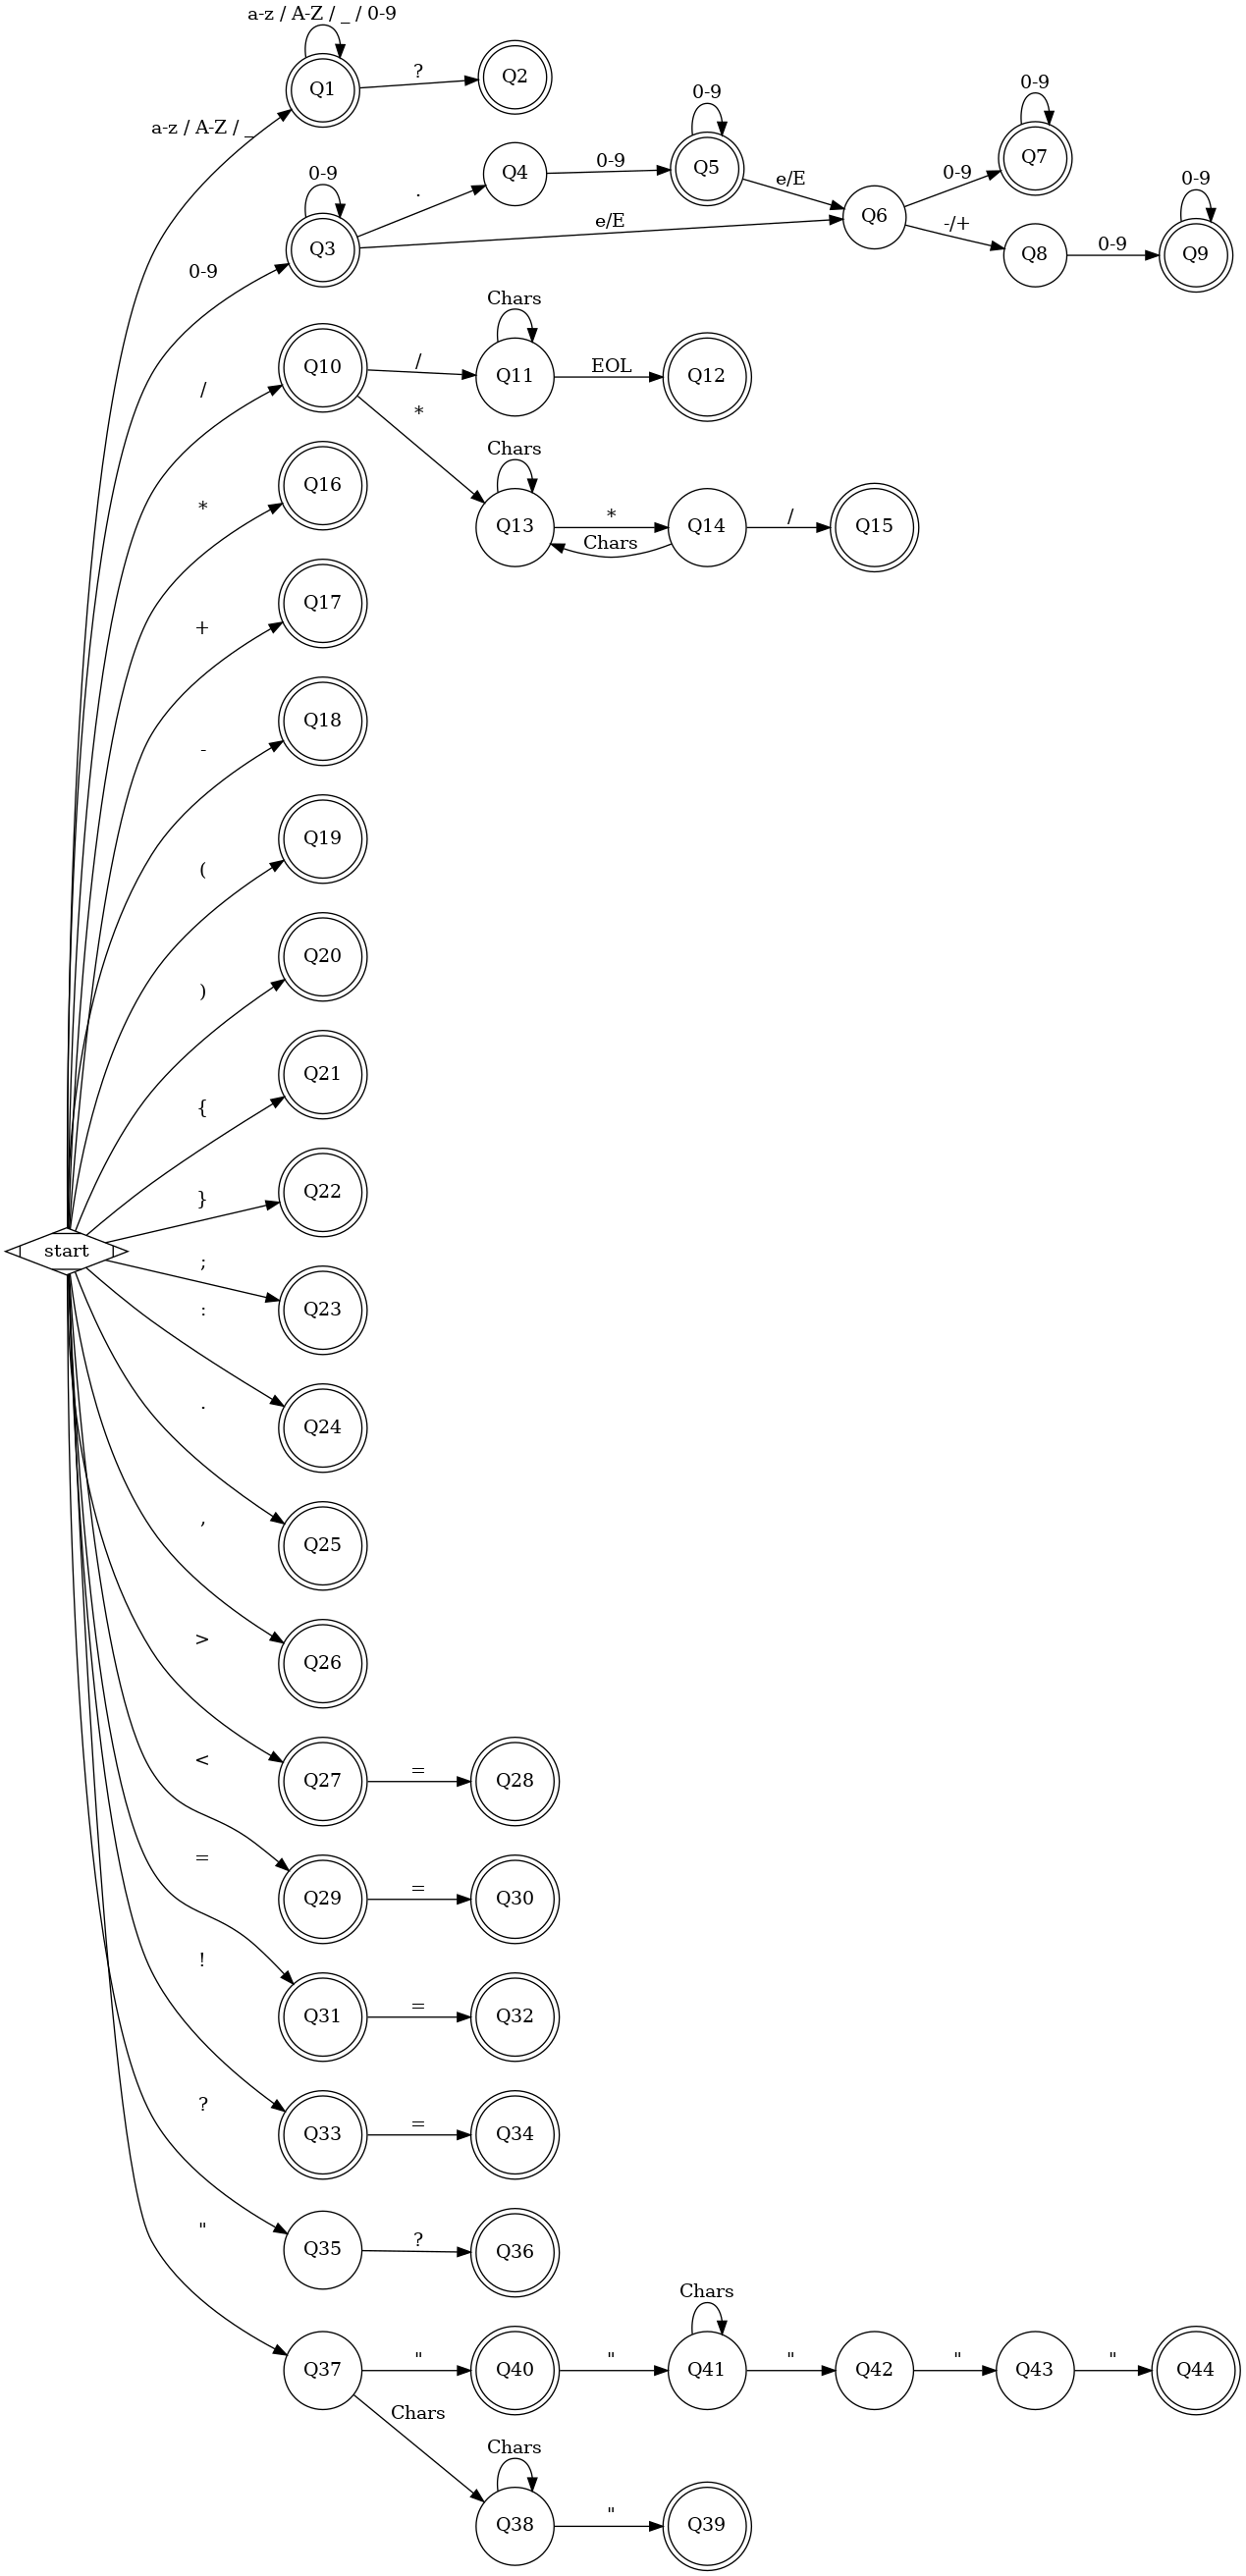
\includegraphics[scale=0.23]{fsm.png}
        \caption{Diagram konečného automatu lexikálního analyzátoru}
        \label{fsm}
    \end{figure}

\newpage

\subsection{Precedenční tabulka syntaktického analyzátoru}
    \label{precedence}
    \begin{table}[ht!]
        \centering
        \begin{tabular}{|>{\columncolor[gray]{0.8}}c|c|c|c|c|c|c|c|c|c|c|c|c|c|c|}
            \hline
            \rowcolor[gray]{0.8}
            & \verb|+| & \verb|-| & \verb|*| & \verb|/| & \verb|==| & \verb|!=| & \verb|<| & \verb|>| & \verb|<=| & \verb|>=| & \verb|ID| & \verb|??| & \verb|!| & \verb|$| \\ \hline
            \verb|+| & \verb|>| & \verb|>| & \verb|<| & \verb|<| & \verb|>| & \verb|>| & \verb|>| & \verb|>| & \verb|>| & \verb|>| & \verb|<| & \verb|>| & \verb|<| & \verb|>| \\ \hline
            \verb|-| & \verb|>| & \verb|>| & \verb|<| & \verb|<| & \verb|>| & \verb|>| & \verb|>| & \verb|>| & \verb|>| & \verb|>| & \verb|<| & \verb|>| & \verb|<| & \verb|>| \\ \hline
            \verb|*| & \verb|>| & \verb|>| & \verb|>| & \verb|>| & \verb|>| & \verb|>| & \verb|>| & \verb|>| & \verb|>| & \verb|>| & \verb|<| & \verb|>| & \verb|<| & \verb|>| \\ \hline
            \verb|/| & \verb|>| & \verb|>| & \verb|>| & \verb|>| & \verb|>| & \verb|>| & \verb|>| & \verb|>| & \verb|>| & \verb|>| & \verb|<| & \verb|>| & \verb|<| & \verb|>| \\ \hline
            \verb|==| & \verb|<| & \verb|<| & \verb|<| & \verb|<| & & & & & & & \verb|<| & \verb|<| & \verb|<| & \verb|>| \\ \hline
            \verb|!=| & \verb|<| & \verb|<| & \verb|<| & \verb|<| & & & & & & & \verb|<| & \verb|<| & \verb|<| & \verb|>| \\ \hline
            \verb|<| & \verb|<| & \verb|<| & \verb|<| & \verb|<| & & & & & & & \verb|<| & \verb|<| & \verb|<| & \verb|>| \\ \hline
            \verb|>| & \verb|<| & \verb|<| & \verb|<| & \verb|<| & & & & & & & \verb|<| & \verb|<| & \verb|<| & \verb|>| \\ \hline
            \verb|<=| & \verb|<| & \verb|<| & \verb|<| & \verb|<| & & & & & & & \verb|<| & \verb|<| & \verb|<| & \verb|>| \\ \hline
            \verb|>=| & \verb|<| & \verb|<| & \verb|<| & \verb|<| & & & & & & & \verb|<| & \verb|<| & \verb|<| & \verb|>| \\ \hline
            \verb|ID| & \verb|>| & \verb|>| & \verb|<| & \verb|<| & \verb|>| & \verb|>| & \verb|>| & \verb|>| & \verb|>| & \verb|>| & & \verb|>| & \verb|>| & \verb|>| \\ \hline
            \verb|??| & \verb|<| & \verb|<| & \verb|<| & \verb|<| & \verb|>| & \verb|>| & \verb|>| & \verb|>| & \verb|>| & \verb|>| & \verb|<| & \verb|<| & \verb|<| & \verb|>| \\ \hline
            \verb|!| & \verb|>| & \verb|>| & \verb|>| & \verb|>| & \verb|>| & \verb|>| & \verb|>| & \verb|>| & \verb|>| & \verb|>| & & \verb|>| & \verb|<| & \verb|>| \\ \hline
            \verb|$| & \verb|<| & \verb|<| & \verb|<| & \verb|<| & \verb|<| & \verb|<| & \verb|<| & \verb|<| & \verb|<| & \verb|<| & \verb|<| & \verb|<| & \verb|<| & \\ \hline
        \end{tabular}
        \caption{Precedenční tabulka syntaktického analyzátoru}
    \end{table}

\newpage

\subsection{LL(1) gramatika syntaktického analyzátoru}
    \begin{verbatim}
01) <start>           -> <program> <end>
02) <end>             -> eps
03) <end>             -> EOF
04) <program>         -> <statement> <program>
05) <program>         -> func FID ( <params> ) <func_type> 
                         { <statement_block> } <program>
06) <program>         -> eps
07) <statement_block> -> <statement> <statement_block>
08) <statement_block> -> eps
09) <func_type>       -> <type>
10) <func_type>       -> eps
11) <params>          -> param_ID ID : <type> <params_n>
12) <params>          -> eps
13) <params_n>        -> , param_ID ID : <type> <params_n>
14) <params_n>        -> eps
15) <type>            -> Int
16) <type>            -> Double
17) <type>            -> String 
18) <statement>       -> return expression
19) <statement>       -> <keyword> ID <var_type> <defvar> 
20) <statement>       -> while ( expression ) { <statement_block> }
21) <statement>       -> if <if_type> { <statement_block> }
                         else { <statement_block> } 
22) <statement>       -> <rvalue> 
23) <statement>       -> ID = <rvalue> 
24) <rvalue>          -> FID ( <args> )
25) <rvalue>          -> expression
26) <args>            -> param_ID : <term> <args_n>
27) <args>            -> <term> <args_n>
28) <args>            -> eps
29) <args_n>          -> , <args_n_final>
31) <args_n>          -> eps
32) <args_n_final>    -> param_ID : <term> <args_n>
32) <args_n_final>    -> <term> <args_n>
33) <term>            -> ID
34) <term>            -> Int_Value
35) <term>            -> String_Value
36) <term>            -> Double_Value
37) <term>            -> nil
38) <if_type>         -> ( expression )
39) <if_type>         -> let ID
40) <defvar>          -> = <rvalue> 
41) <defvar>          -> eps
42) <keyword>         -> var
43) <keyword>         -> let
44) <var_type>        -> : <type>
45) <var_type>        -> eps
    \end{verbatim}
    \label{ll-grammar}

\newpage

\section{Literatura}
\bibliographystyle{czechiso}
\renewcommand{\refname}{}
\bibliography{dokumentace}

\end{document}
